\documentclass[10pt,a4paper]{extarticle}
\usepackage[a4paper, margin=1in]{geometry}
\usepackage{graphicx, float, xcolor}
\usepackage{setspace, titlesec, fontspec, enumitem}
\usepackage{array, multicol, tocloft, longtable, booktabs}


\setlength{\parindent}{0pt}    
\setlength{\parskip}{6pt}
\onehalfspacing

\setmainfont[
  Path = ./fonts/,
  UprightFont = *-Regular,
  BoldFont = *-Bold,
  ItalicFont = *-Italic,
  BoldItalicFont = *-BoldItalic
]{Mulish}


\begin{document}

\begin{titlepage}
    \centering
    
\includegraphics[width=4cm]{figures/uap logo.png}\par
    \vspace{1cm}
    
    {\Huge\bfseries University of Asia Pacific\par}
    \vspace{0.5cm}
    {\Large Peripheral \& Interfacing Lab\par}
    \vspace{.3cm}
    {\large Course code: \textbf{CSE 316}\par}
    
    \vspace{2cm}
    {\Huge\color{blue!40!black} \textbf{Pawmigo}\par}
    \vspace{0.3cm}
    {\large (Smart Cat Feeder)\par}
    
    \vspace{2cm}
    {\large \textbf{Submitted to}\par}
    \vspace{0.3cm}
    {\large Atia Rahman Orthi\\}
    {\large Lecturer, Department of CSE,\\}
    {\large University of Asia Pacific\\}
    
    \vspace{2cm}
    {\large \textbf{Submitted By}\par}
    
    \vspace{0.5em}
   \begin{center}
   \begin{tabular}{lr}
      \textbf{Name} & \textbf{Registration ID} \\[1em]
      Shahriar Arefin & 22101040 \\[0.5em]
      Mohotasir Al Mamun & 22101036 \\[0.5em]
      Umme Kulsum Surovi & 22101043
   \end{tabular}
\end{center}

\end{titlepage}

\tableofcontents
\thispagestyle{empty}
\newpage

\section{Introduction}

Proper nutrition and care for pets are critical for their health and well-being. Some pets, like dogs and cats, are considered family members; ensuring they receive the correct food in appropriate quantities is essential. However, busy schedules often lead to inconsistent feeding practices, resulting in issues such as underfeeding or overfeeding. Overfeeding can cause obesity, while underfeeding can lead to malnutrition, both of which have significant health implications. Pet food costs are significant for many families, making efficient and controlled feeding practices even more important.
To address these challenges, we aim to develop an automatic pet feeder that uses Internet of Things (IoT) technology and a custom app. The device is designed to dispense appropriate food portions, enhancing pet nutrition management and overall health. By automating the feeding process, the system ensures that pets receive the right amount of food, regardless of the owner's availability. This approach contributes to improving pets' health and well-being and offers pet owners convenience and peace of mind. The development of smart devices for pet feeding has been a growing area of interest due to the need to improve efficiency and effectiveness in pet feeding. Additionally, integrating a custom app has proven effective in enhancing monitoring and control systems .This project aims to design and develop a smart pet feeder that combines IoT and deep learning technologies to automatically and accurately dispense food. This project addresses common issues such as overfeeding and underfeeding and enhances convenience for pet owners, ensuring their pets receive the necessary care even in their absence.

Pawmigo is an IoT-based smart cat feeder designed to provide pet owners with a convenient and automated way to feed their cats. The system uses an ESP8266 microcontroller to enable remote feeding scheduling, portion control, and real-time monitoring via a mobile app or web interface. In modern urban life, many pet owners, especially cat owners, have busy schedules that make it challenging to feed their pets on time. Proper feeding schedules are crucial for a pet's health, but owners may miss feeding times due to work commitments, travel, or other responsibilities. To solve this problem, our team is developing a “Smart Pet Feeder”, an automated system that ensures pets receive food on time, even when their owners are away. 

\vspace{2em}


\begin{figure}[H]
   \centering
   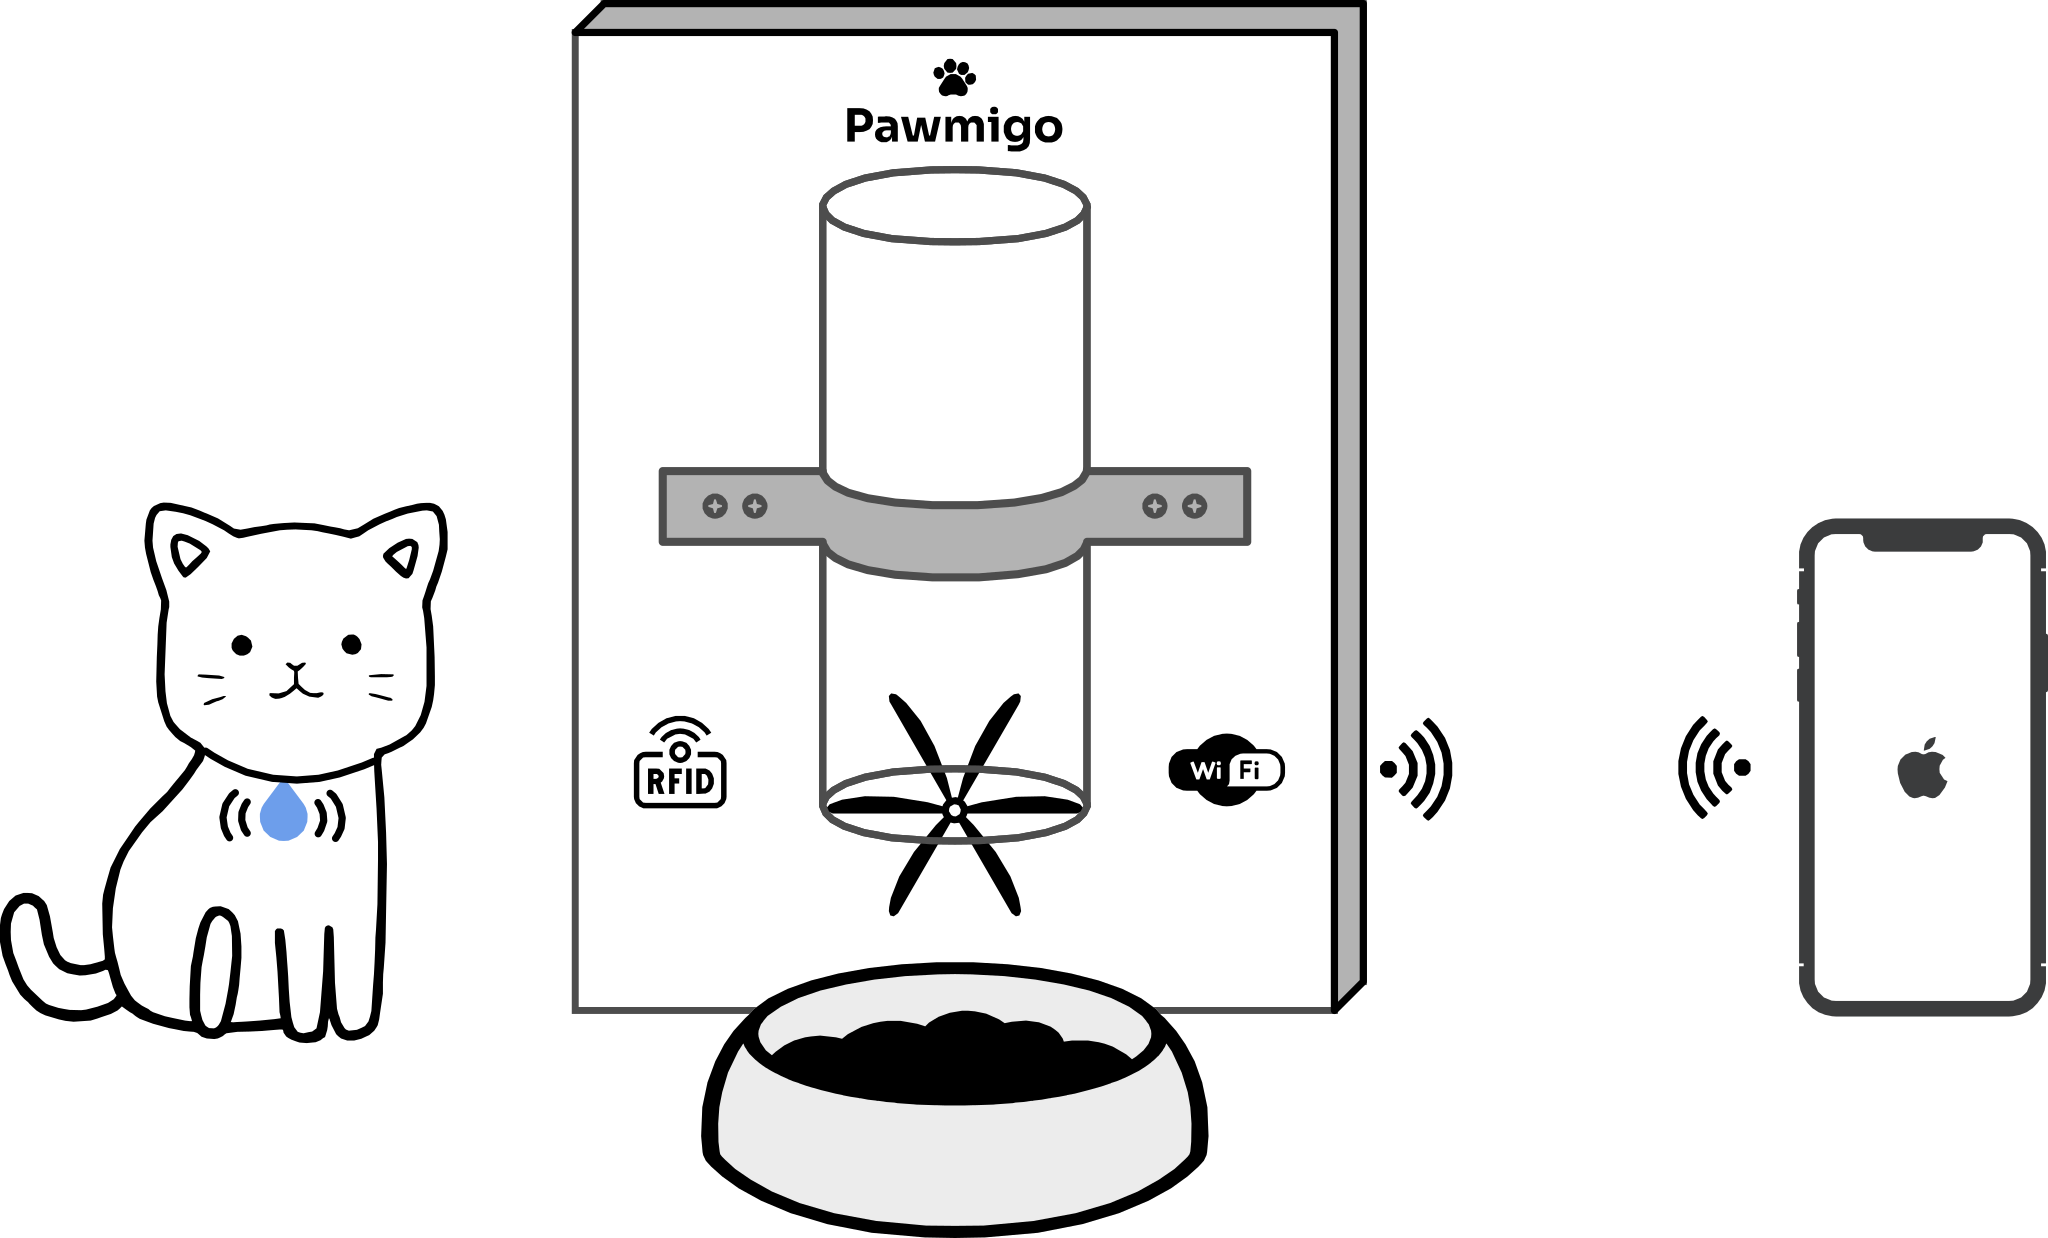
\includegraphics[width=0.8\textwidth]{figures/Pawmigo.png}
   \label{fig:pawmigo}
\end{figure}

\newpage
\section{Objective}

The primary objective of the “Pawmigo” smart pet feeder project is to design and develop a reliable, user-friendly, and cost-effective automated feeding system specifically tailored for cats. The system aims to support pet owners by ensuring timely and measured food dispensing regardless of their physical availability, while also providing essential monitoring and control features through IoT-based technology.

Imagine a cat owner who works long hours and has an irregular schedule. He needs a reliable way to feed his cat four times a day without manual intervention. Our Pawmigo allows him to set feeding schedules through a mobile app, ensuring that food is dispensed at the exact time. The system consists of three main components: Food Dispenser – Stores and releases food at scheduled times. The mobile app allows the owner to set feeding times and manually dispense food if needed. Sensors (including RFID) - Detects when the cat is near and enables additional feeding control.  At the scheduled feeding times, the dispenser automatically releases food, ensuring the cat gets its meals regularly. However, in some cases, the cat may feel hungry outside of the scheduled times and approach the feeder for extra food. To handle this, we integrate an RFID sensor with the cat's collar. When the cat comes near the feeder, the system detects its presence and sends a notification to the owner's mobile app, asking: "Your cat is near the feeder. Would you like to dispense more food?" The owner can then decide whether to allow additional feeding, preventing underfeeding or overfeeding.


The project focuses on achieving the following specific objectives:

\begin{enumerate}
    \item \textbf{Automated Feeding with Scheduled Control:} To implement a scheduling mechanism that allows pet owners to pre-define feeding times and food quantities through a mobile app or web interface. This ensures that pets are fed consistently, even in the absence of the owner.
    
    \item \textbf{Remote Access and Monitoring:} To provide real-time interaction with the feeder using an ESP8266 microcontroller connected to a Wi-Fi network. The system should allow users to view the feeder status, track feeding history, and trigger manual feeding remotely.
    
    \item \textbf{Portion Management and Health Awareness:} To regulate the amount of food dispensed during each feeding session to prevent overfeeding or underfeeding. Controlled portions contribute to maintaining the pet's health, reducing obesity, and promoting a balanced diet.
    
    \item \textbf{Pet Detection and Owner Notification:} To incorporate an RFID-based detection mechanism that identifies when the pet approaches the feeder outside the scheduled feeding time. When detected, the system will notify the owner, helping them understand the pet's habits and hunger patterns.
    
    \item \textbf{Low-Cost and Scalable Hardware Architecture:} To design a system that uses readily available and affordable components such as ESP8266, servo or stepper motors, RFID readers, and buzzers. This allows for ease of assembly, maintenance, and potential scalability or customization in the future.
    
    \item \textbf{User-Friendly Interface:} To develop an intuitive user interface that allows seamless communication between the owner and the feeder system. Whether through a dedicated mobile application or a web portal, the interface should be secure, responsive, and easy to use.
    
   %  \item \textbf{User-Friendly Interface with Custom Mobile App:} To develop an intuitive, custom-built mobile application that allows seamless communication between the pet owner and the feeder system. The app enables users to set feeding schedules, trigger manual feedings, and receive real-time notifications (e.g., when the cat approaches the feeder). The interface is designed to be secure, responsive, and easy to use, ensuring accessibility and convenience for the owner at all times.

   %  \item \textbf{Improved Pet-Care Experience:} To enhance the overall experience of pet ownership by reducing stress, building routine, and allowing owners to focus on other responsibilities without compromising their pet's dietary needs.
\end{enumerate}


\vspace{8pt}

\section{Methodology}

The development of the Smart Pet Feeder, follows a structured methodology involving the design, implementation, and integration of hardware and software components. The approach focuses on building a reliable, low-cost system that meets the needs of modern cat owners by automating feeding schedules and enabling remote interaction. The methodology is divided into the following key stages:

The table below outlines the development of our project following \textbf{Agile Principles}, breaking work into iterative and incremental steps.

\begin{center}
   \renewcommand{\arraystretch}{1}
   \begin{longtable}{@{} p{3cm} p{12cm} @{}}
      \toprule
      \textbf{Step} & \textbf{Work Description} \\
      \midrule
      \textbf{Step 1} & Finalized the project concept and prepared the official project proposal. \\[5pt]
      \textbf{Step 2} & Identified, sourced, and collected all necessary hardware components. \\[5pt]
      \textbf{Step 3} & Connected and tested hardware components for initial integration. \\[5pt]
      \textbf{Step 4} & Completed the mobile application development. \\[5pt]
      \textbf{Step 5} & Integrated hardware and software for full system operation. \\[5pt]
      \textbf{Step 6} & Finalized development of the mobile application. \\
      \bottomrule
   \end{longtable}
\end{center}

\vspace{-\baselineskip}
\subsection{Development Approach}
The development approach is based on a modular and iterative design, allowing for gradual development, testing, and improvement. The first stage involves requirement analysis and planning, where we define the essential features needed to address common pet owner challenges, such as automatic feeding, real-time monitoring, and remote food dispensing. A detailed system architecture is designed, incorporating the food dispenser, sensors, and mobile application. Once the fundamental requirements are established, we move to the prototyping phase, where initial hardware testing is conducted to ensure the food dispenser mechanism operates correctly. Simultaneously, the software design is structured, including the development of the mobile app's user interface (UI) and backend server functionality. The project follows an \textbf{'Agile methodology'}, where features are developed in small increments, thoroughly tested, and refined based on feedback. This ensures continuous improvements, allowing us to enhance user experience and system reliability before the final deployment.


\subsection{System Overview}
The following diagram illustrates the overall structure of the Smart Pet Feeder system, showing the interaction between hardware components and the mobile application.

The system is composed of three primary subsystems:
\begin{itemize}
    \item \textbf{Food Dispensing Mechanism:} A motor-driven container that releases food at predefined times.
    
    \item \textbf{Control and Connectivity Module:} Powered by the ESP8266 microcontroller, which handles scheduling, user commands, and Wi-Fi communication.
    
    \item \textbf{User Interface:} A custom mobile application through which users can set schedules, receive notifications, and control feeding remotely.
\end{itemize}

\begin{figure}[H]
   \centering
   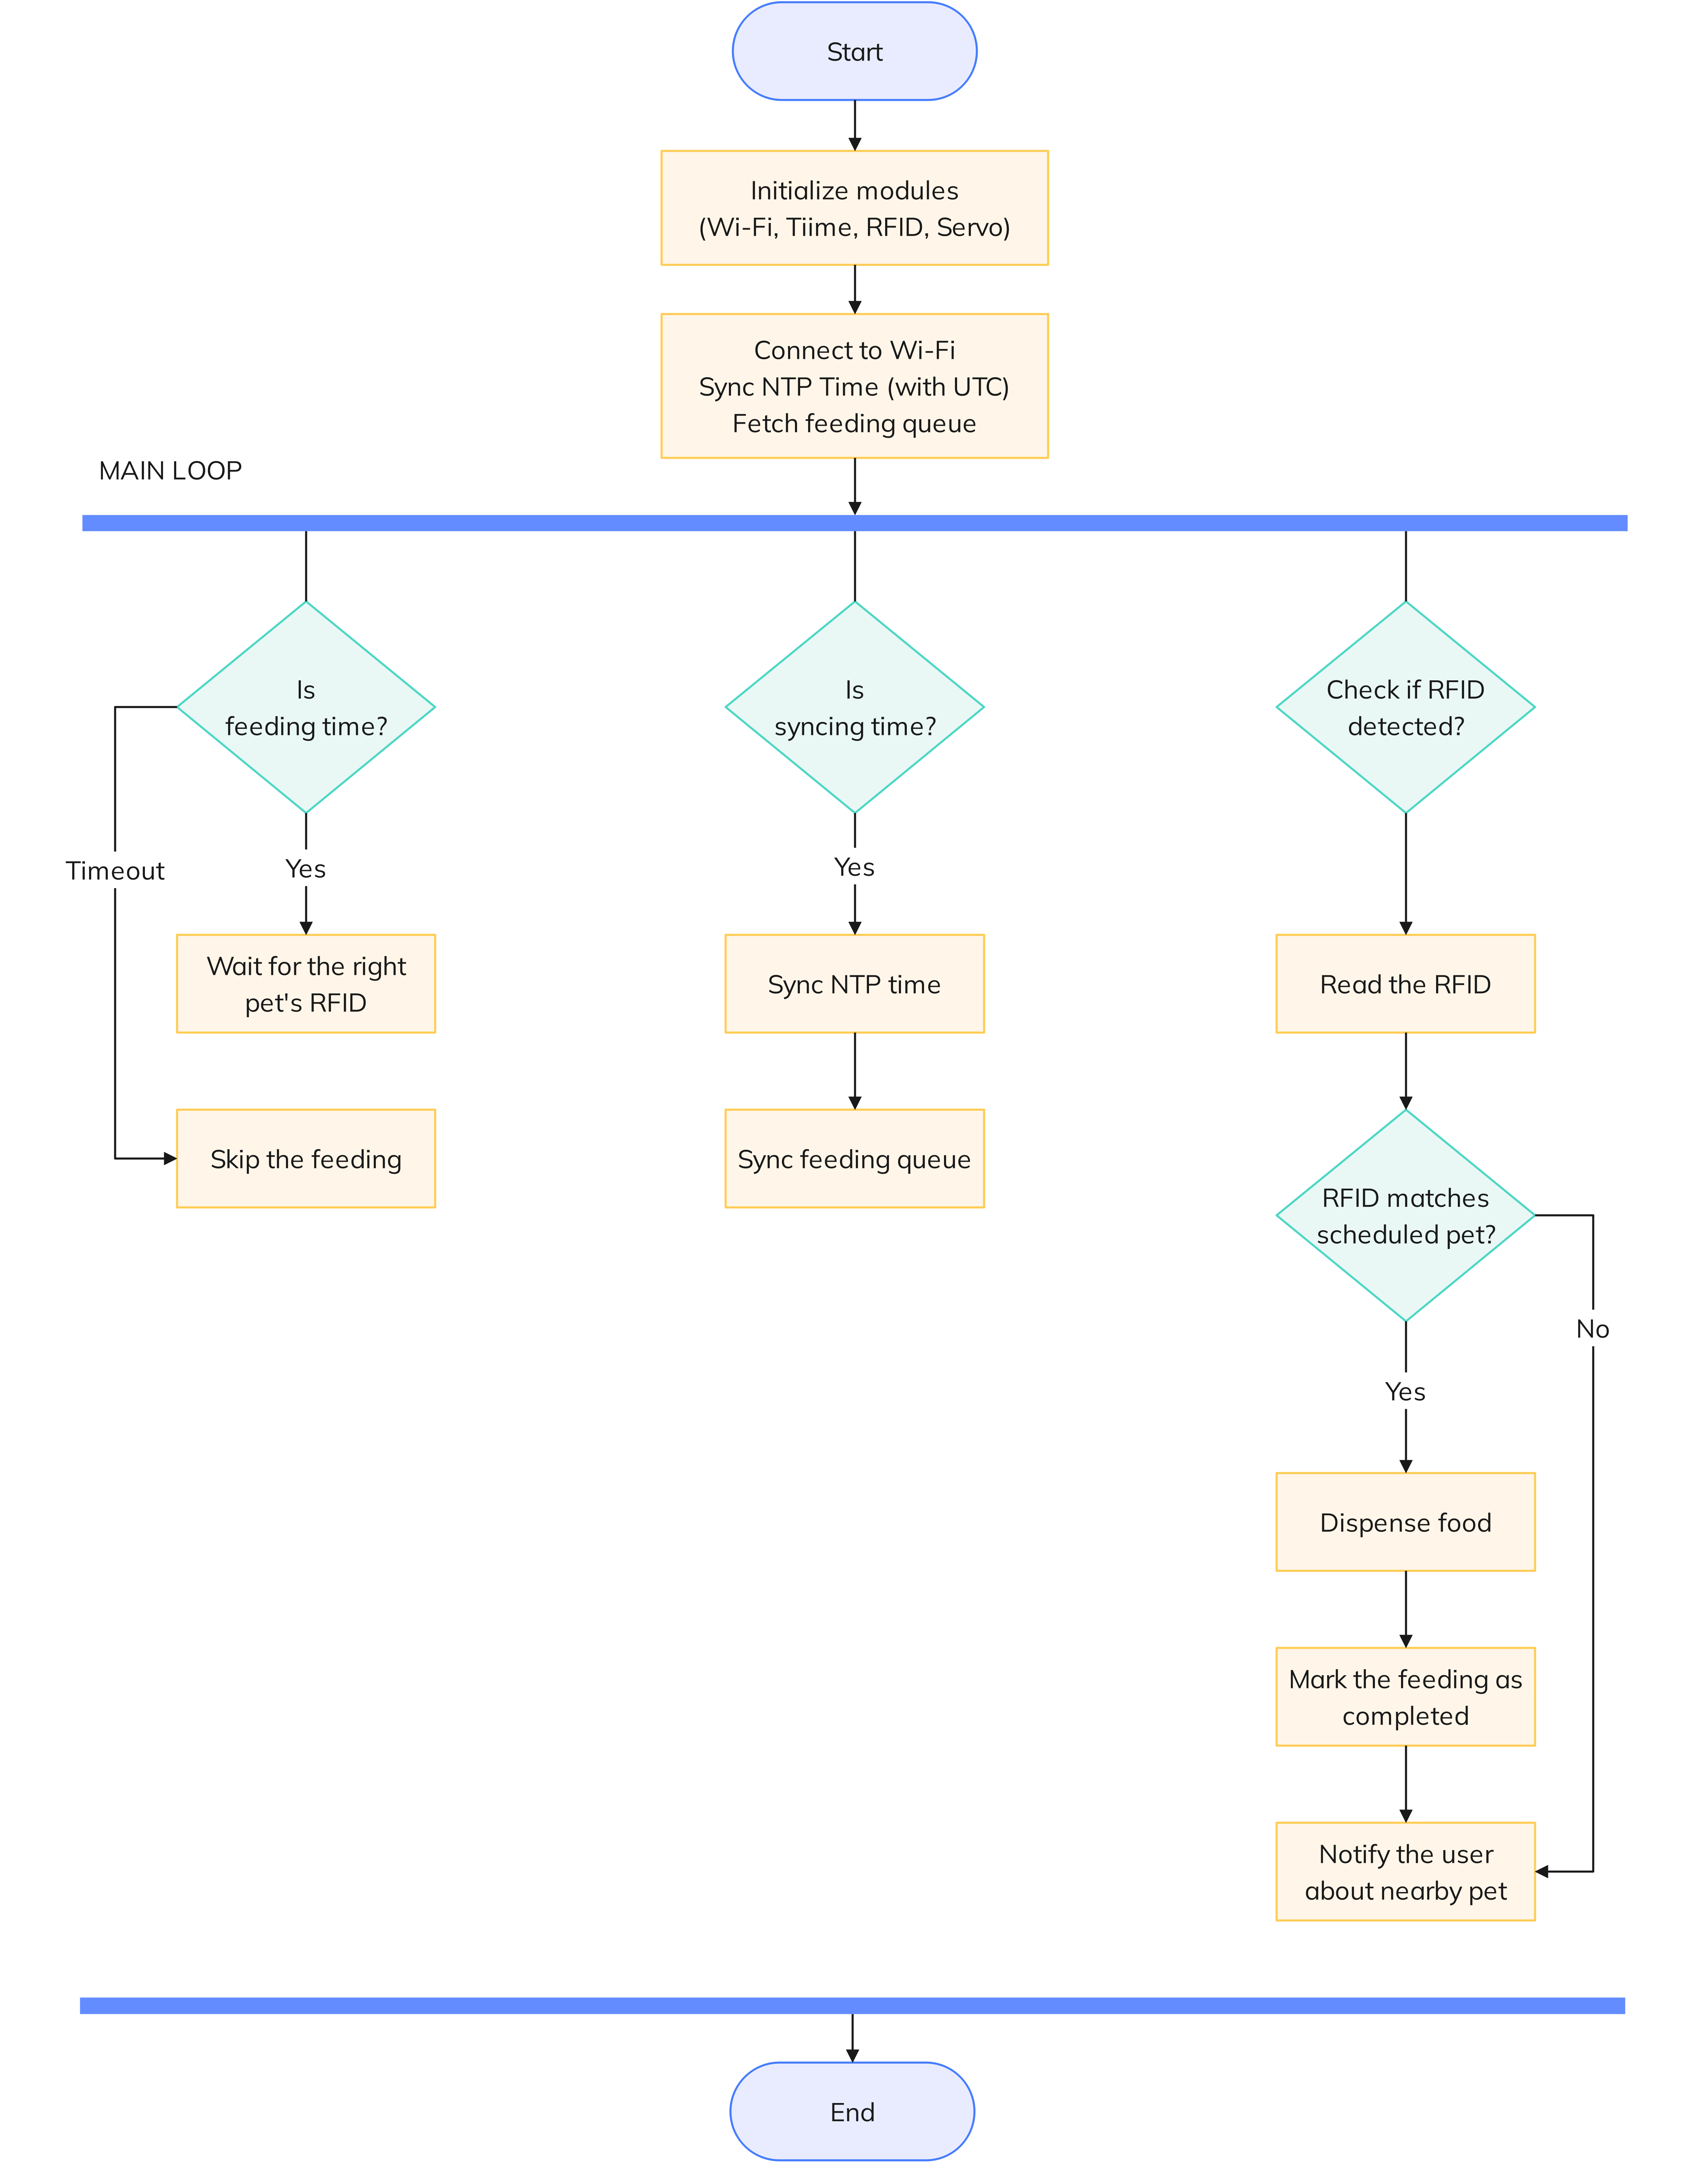
\includegraphics[width=\textwidth]{figures/Pawmigo System.png}
   \caption{Pawmigo Working Procedure}
   \label{fig:architecture}
\end{figure}




\subsection{Hardware Design}
The hardware design includes the selection and integration of electronic and mechanical components required to automate the feeding process:

\vspace{-0.5\baselineskip}
\begin{table}[H]
   \renewcommand{\arraystretch}{1.5}
   \begin{longtable}{@{}p{5cm}p{10cm}@{}}\toprule
      \textbf{Component} & \textbf{Description} \\\midrule
      ESP8266 Microcontroller & Serves as the core of the system, managing all operations. \\
      
      RFID Module & Detects the cat's presence using a tag on its collar. \\
      
      SG90 Servo Motor $\times$ 2 & Helps in food dispensing food. \\
      
      Breadboard & Used to prototype and connect electronic components. \\
      
      Cables \& Wires & Used for connecting all components within the system.\\
      
      Buzzer & Provides audible feedback for different operations. \\
      
      Power Supply & Provides stable 3.3V or 5V power to all components. \\
      
      Ultrasonic Sensor & Used to detect the food level. \\
      
      HW-131 power supply & Provides stable power to the breadboard. \\

      18650 battery & Provides power to the system.
      \\\bottomrule
   \end{longtable}
\end{table}



\subsection{Software Architecture}
The software is divided into firmware running on the ESP8266 and a mobile app developed by the team:
\begin{itemize}
    \item \textbf{ESP8266 Firmware:} Written in C++ using Arduino IDE. It connects to Wi-Fi, receives instructions from the app, and executes the feeding schedule.
    \item \textbf{Custom Mobile App:} To enhance user accessibility and remote control capabilities, we developed a custom mobile application as part of our smart pet feeder system. The app was built using React Native, allowing us to create a cross-platform application that runs smoothly on both Android and iOS devices.

For the user interface (UI), we implemented Tailwind CSS, which provides a utility-first styling approach. This enabled us to rapidly design a clean, responsive, and modern interface, optimizing the user experience for mobile interaction
    \item \textbf{Backend Services (if any):} We use Convex as a  database to store log feeding data or backup schedule settings.
\end{itemize}

\subsection{Feeding Schedule and Portion Control Logic}

Users define feeding times and portion sizes in the mobile app. These are transmitted to the ESP8266, which stores them in memory or EEPROM. At scheduled times:

\vspace{-0.5\baselineskip}
\begin{enumerate}[parsep=0em]
    \item The motor is activated to release a measured amount of food.
    \item The system confirms the feeding operation and updates the status.
    \item A notification can be sent to the app to confirm food delivery.
\end{enumerate}

This ensures consistent and timed feeding even if the internet is temporarily unavailable, as the schedule can be preloaded onto the device.

\subsection{RFID Detection and Owner Notification}

To handle unscheduled hunger events:
\begin{itemize}[parsep=0em]
    \item An RFID reader detects the pet's presence when it comes near the feeder.
    \item The system sends a real-time alert to the mobile app.
    \item The owner receives a message such as “Your cat is near the feeder. Dispense more food?”
    \item The owner can respond through the app to either approve or deny extra feeding.
\end{itemize}

This feature helps avoid both underfeeding and overfeeding by involving the owner in real-time decision-making.

\subsection{Testing and Validation}
The final prototype undergoes testing in multiple phases:

\begin{itemize}
    \item \textbf{Component Testing:} Verifying individual components like the motor, RFID reader, and buzzer.
    \item \textbf{Integration Testing:} Ensuring that the ESP8266 interacts correctly with both hardware and the mobile app.
    \item \textbf{Real-World Simulation:} Testing the system in a home-like environment with a real or simulated cat to verify schedule accuracy, notifications, and reliability.
\end{itemize}

Issues found during testing are documented and resolved iteratively until the system achieves reliable performance.

\pagebreak
\section{Budget}

The table below outlines the total cost of components used in the development of the Smart Pet Feeder (Pawmigo) system. The focus was to build a low-cost, efficient prototype using readily available components. All prices are in Bangladeshi Taka (BDT).

\begin{table}[H]
\centering
\renewcommand{\arraystretch}{1.4}
\begin{tabular}{|c|l|c|}
\hline
\textbf{Sl. No.} & \textbf{Component} & \textbf{Cost (BDT)} \\
\hline
1 & ESP8266 Microcontroller & 300 \\
2 & RFID Module & 150 \\
3 & 28BYJ-48 Stepper Motor with ULN2003 Driver & 230 \\
4 & SG90 Servo Motor $\times$ 2 & 280 \\
5 & Ultrasonic Sensor & 100 \\
6 & Breadboard  & 260 \\
7 & Cables \& Wires & 100 \\
8 & 18650 battery $\times$ 2 & 200 \\
9 & 18650 battery holder & 50 \\
10 & Breadboard power supply module & 80 \\
\hline
\multicolumn{2}{|r|}{\textbf{Total}} & \textbf{1750} \\
\hline
\end{tabular}
\caption{Component-wise Budget Breakdown}
\end{table}

The total expenditure for building the prototype system amounts to \textbf{1750 BDT}. The cost may vary slightly depending on market availability or sourcing methods. All components were chosen to maintain an effective balance between affordability and performance.


\section{Result \& Discussion}
The Smart Pet Feeder system was successfully designed, developed, and tested. The final prototype demonstrated reliable functionality across all planned features, meeting the core objectives of automated feeding, remote access, and real-time monitoring. The following results were observed during testing and demonstration phases:

\subsection{Automated Feeding Performance}
The scheduled feeding mechanism worked accurately and consistently. The feeder was able to dispense food at the correct times as defined by the user through the mobile app. Tests conducted over a one-week period with four feeding events per day showed 100\% success in food dispensing without motor failure or delay.
\begin{itemize}[parsep=0em]
    \item Food dispensing was accurate within ±5 grams per portion.
    \item Feeding times remained consistent even after power resets (due to EEPROM schedule storage).
    \item Manual feeding triggered from the mobile app responded within 2–3 seconds on average.
\end{itemize}

\subsection{Mobile Application Integration}
The custom-built mobile application allowed seamless communication with the ESP8266 microcontroller. Users were able to:
\begin{itemize}[parsep=0em]
    \item Set and modify feeding schedules.
    \item Trigger manual feeding remotely.
    \item Receive real-time alerts and confirmations.
\end{itemize}

The app was tested on both Android and iOS devices and maintained stable performance with no crashes during operation.

\subsection{RFID Detection and Notification System}

The RFID based detection system successfully identified when the tagged cat approached the feeder. The ESP8266 responded by sending notifications to the mobile app in real-time. The response time was typically less than 3 seconds, depending on the Wi-Fi connection.

\begin{itemize}[parsep=0em]
    \item Detection range of RFID reader: Approximately 5–7 cm.
    \item False detection rate: 0\% during controlled testing.
    \item Notification prompt allowed the owner to decide on additional feeding, adding a layer of control to prevent overfeeding.
\end{itemize}

\subsection{System Stability and Power Management}

The feeder operated continuously for 7 days during the testing phase without system crashes or communication failures. A regulated 5V power supply ensured stable operation of both the ESP8266 and motor driver.

\begin{itemize}[parsep=0em]
   \item System uptime during test phase: 100\%
   \item No memory overflow or software glitches were encountered
   \item Power consumption was within acceptable limits for home use
\end{itemize}

\subsection{User Feedback}

Informal testing with a few users (pet owners) was conducted to gather feedback on usability and interface design. The feedback included:

\begin{itemize}[parsep=0em]
    \item Easy-to-use interface with minimal learning curve.
    \item Users appreciated the ability to monitor feeding history.
    \item Notification system was helpful for decision-making during irregular hunger events.
\end{itemize}

Overall, the results confirm that the Smart Pet Feeder meets its functional requirements and is ready for further refinement or scaling.

\newpage

\section{Conclusion}
In this project, we developed Pawmigo, a smart pet feeder that automates and streamlines the feeding process using RFID and WiFi connectivity. By integrating an RFID sensor, the system can notify the cat owner if he/she wants to feed his/her cat manually. A servo-motor-controlled food dispenser precisely releases a predefined portion of food, ensuring proper portion control. The ESP8266 WiFi module enables remote access through a mobile app, allowing pet owners to schedule feedings, manually dispense food, and monitor feeding history from anywhere.

This system offers significant benefits to cat owners by providing a convenient, automated, and controlled feeding solution. It eliminates the need for manual feeding, ensures pets are fed on time, and allows remote monitoring for busy or traveling owners. Additional features like portion control, multiple pet access, and potential health tracking make it an ideal solution for maintaining a pet's health and well-being. With Pawmigo, cat owners can ensure their pets are properly fed while having peace of mind and greater control over their pet's nutrition.
\end{document}
